We can mathematically model \textbf{logistic growth} by modifying our equation for exponential growth (Equation (\ref{eq:lin1})), using an $r$ (per capita growth rate) that depends on population size $N$ and how close it is to \textbf{carrying capacity} $K$.
\begin{equation}
	\frac{dN}{dt}=rN(1-\frac{N}{K})\quad\rightarrow\quad N(t)=\frac{K}{1+\left(\frac{K-N_0}{N_0}\right)e^{-rt}}
\end{equation}
It can also be written in continuous form as shown above.\\
For any initial value $N_0$, $N\rightarrow K$ as $t\rightarrow\infty$.
\begin{figure}[h!]
	\centering
	\begin{subfigure}{0.38\linewidth}
		\raggedleft
		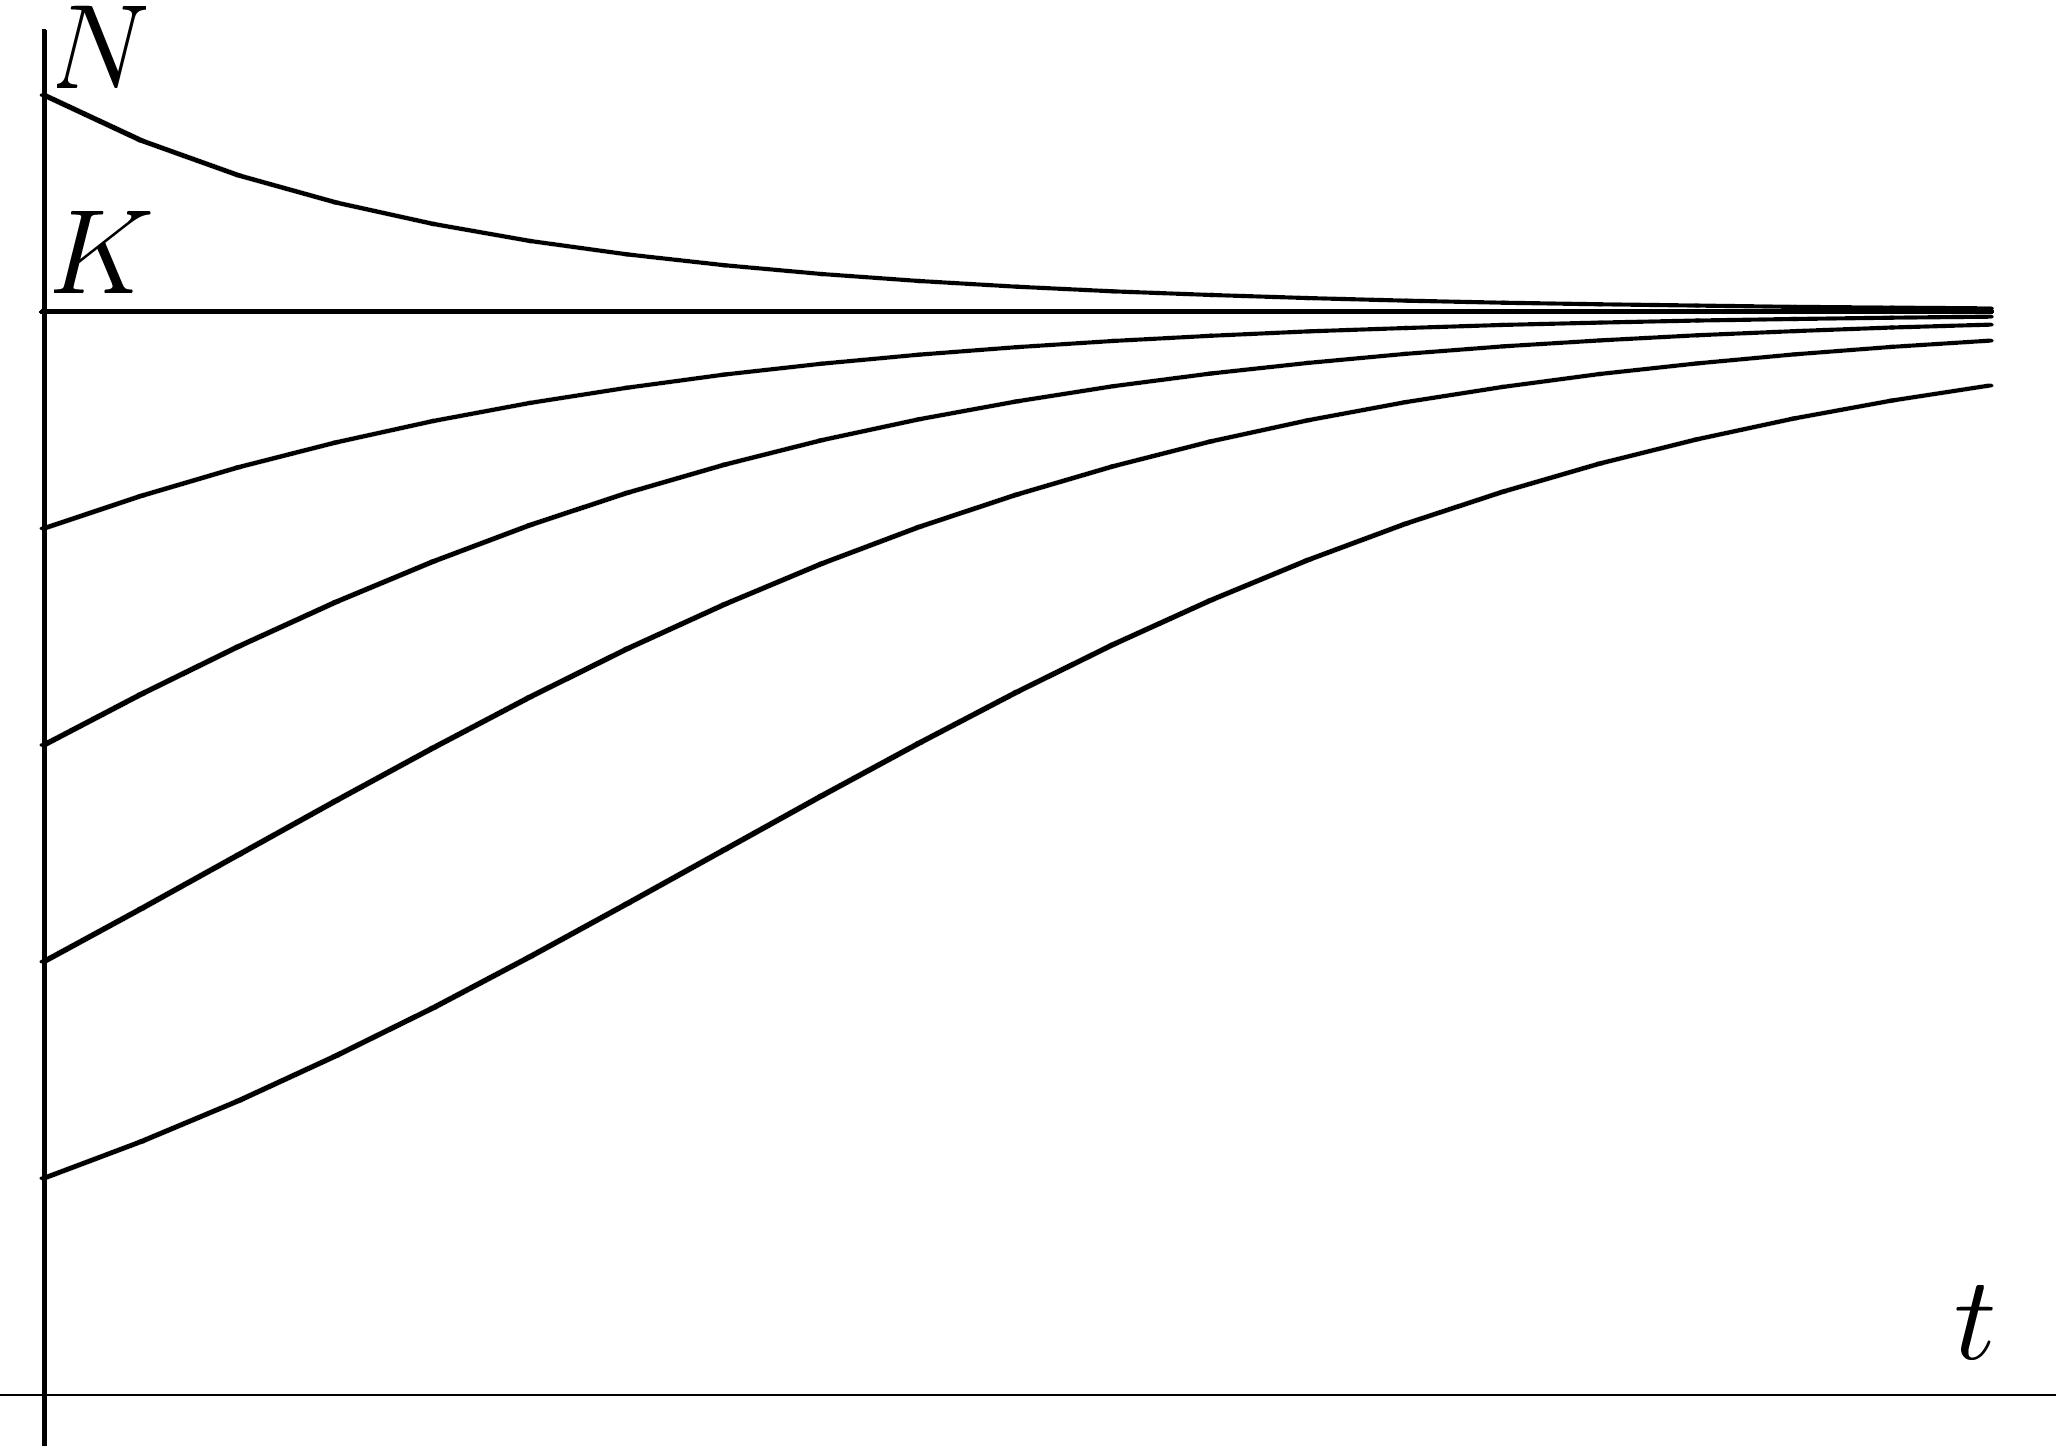
\includegraphics[width=0.689\linewidth]{lg.png}
		\caption{\raggedleft Solutions to Logistic Equation.}
		\label{fig:lg}
	\end{subfigure}
	\vline
	\begin{subfigure}{0.42\linewidth}
		\raggedright
		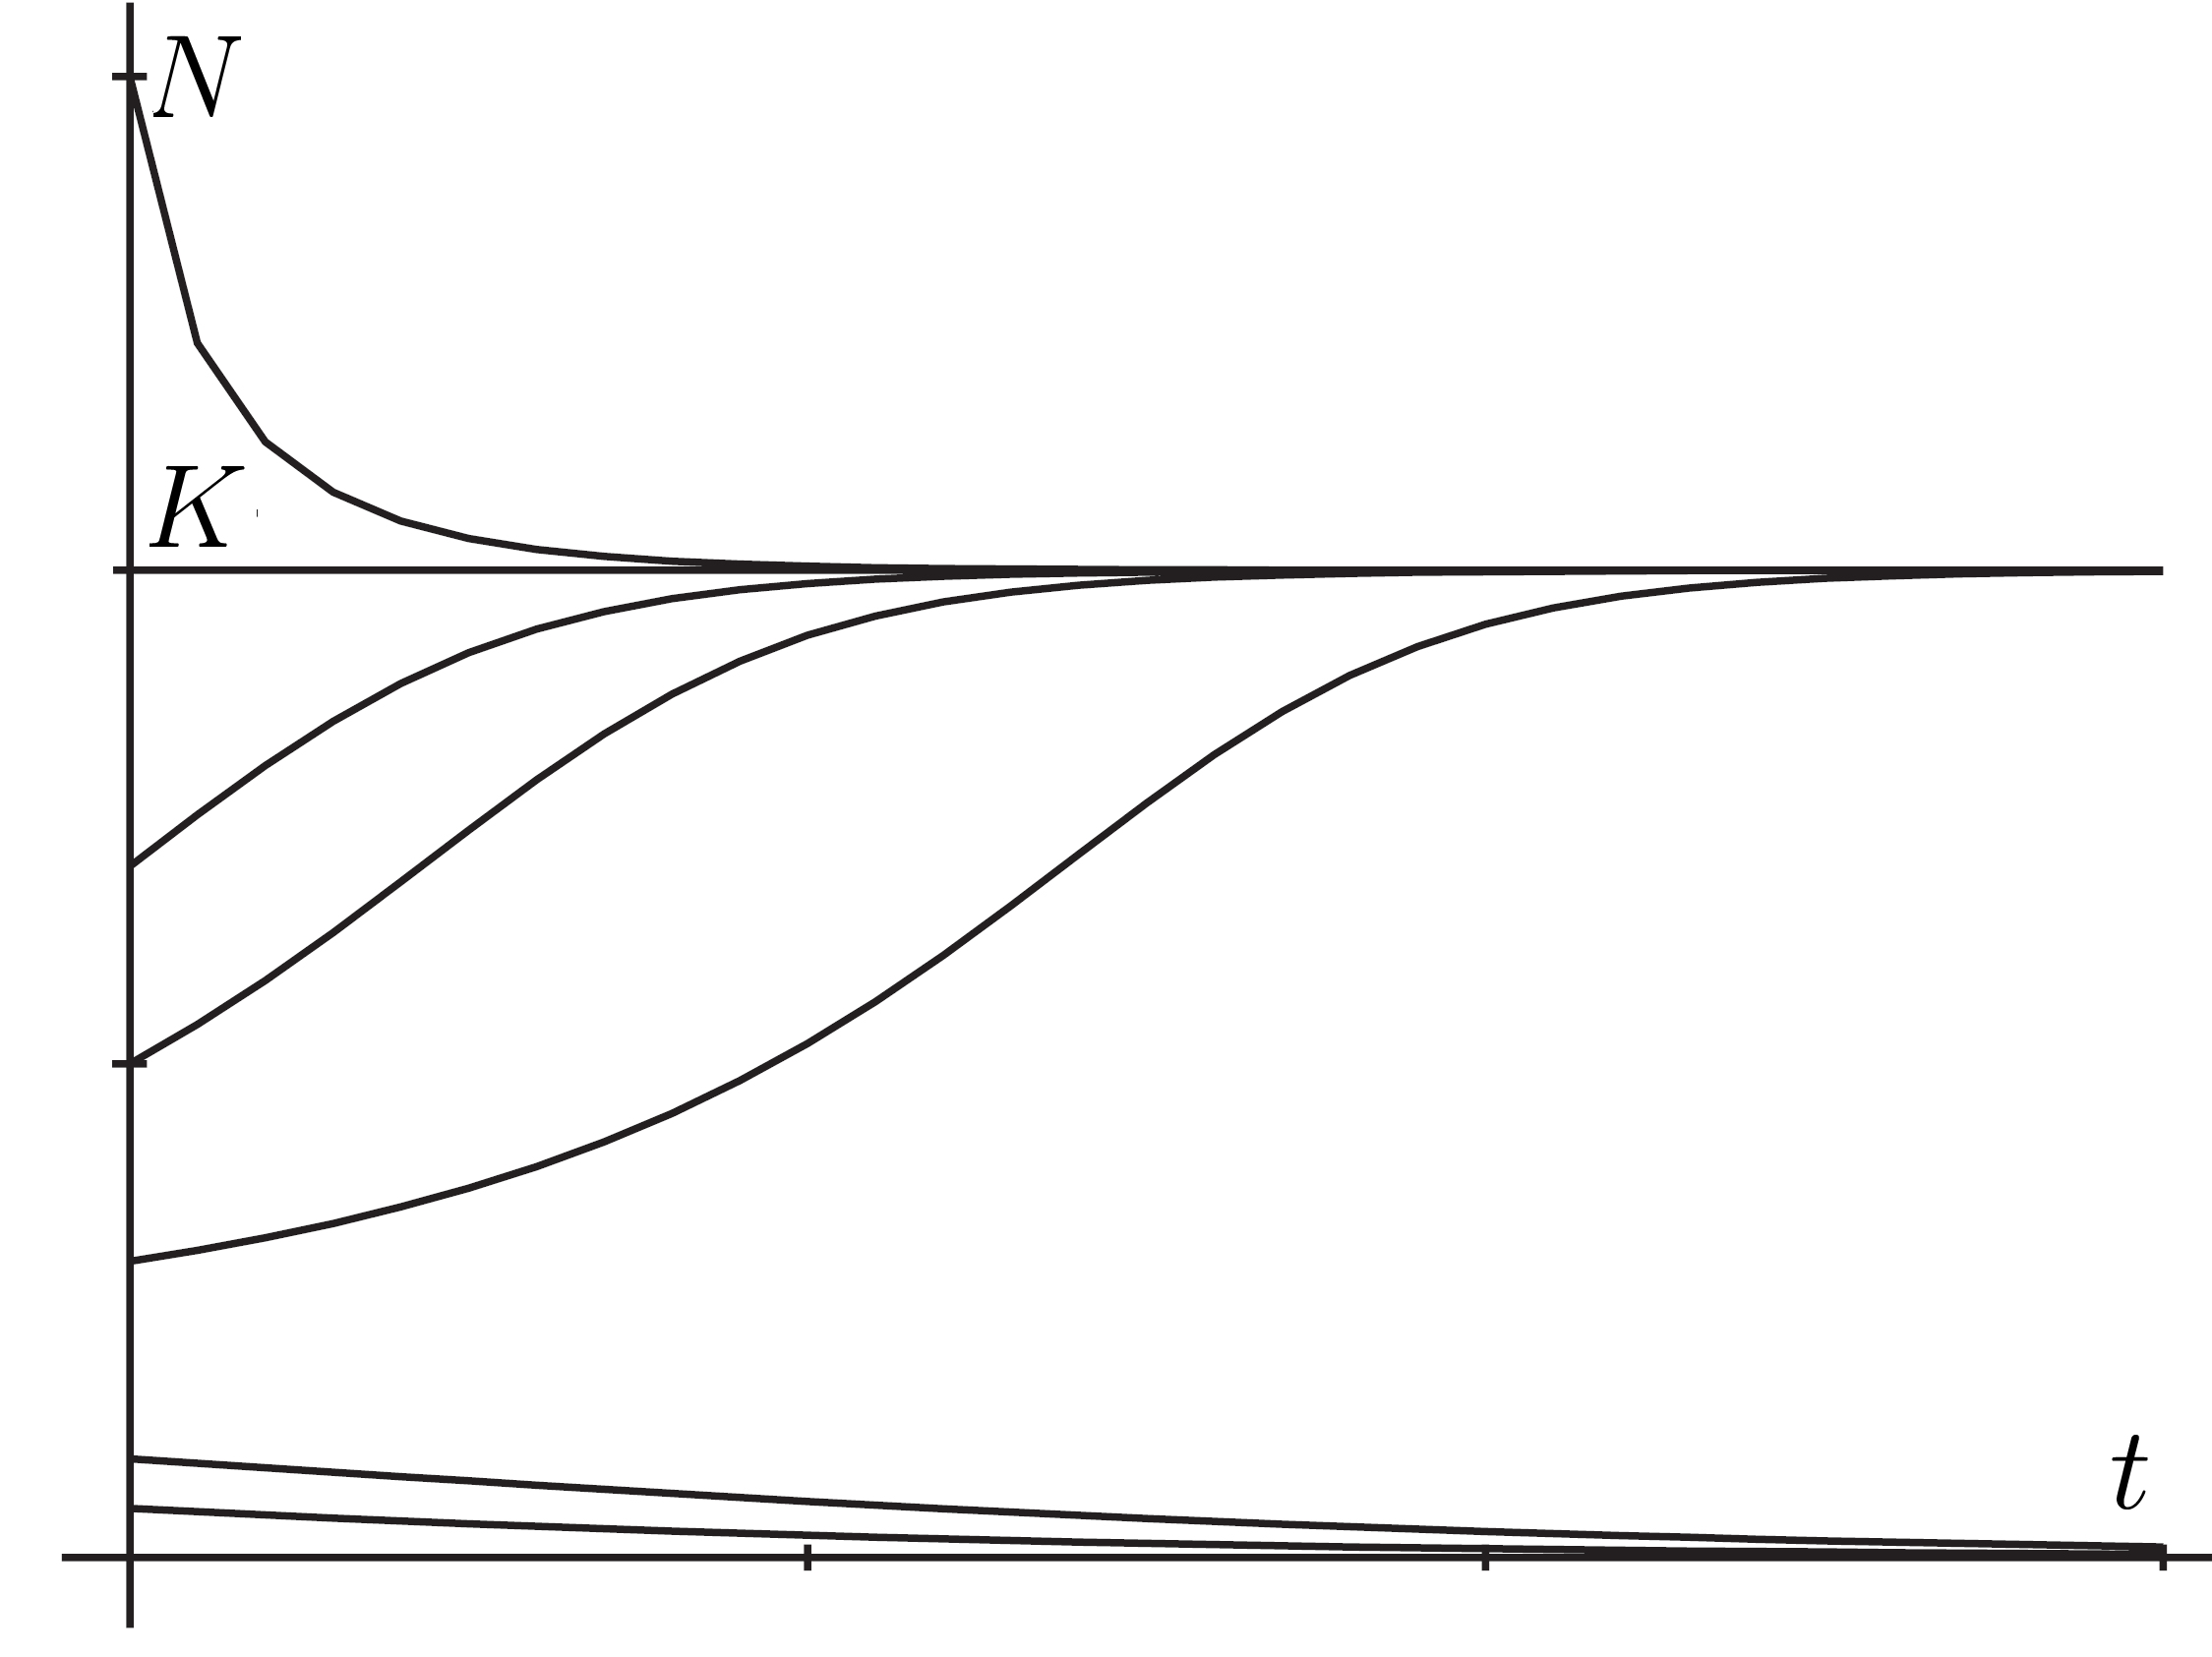
\includegraphics[width=0.59\linewidth]{lgm.png}
		\caption{\raggedright Solutions to the Predator Pit Equation.}
		\label{fig:lgm}
	\end{subfigure}
\end{figure}
Real populations are in danger of extinction if their size falls to a low level.
Predation might eliminate the last few members completely, finding mates becomes more difficult, and lack of genetic diversity renders the population susceptible to epidemics.
We following modification of the logistic equation by constructing a per capita growth rate that is actually negative below some critical value $T$.
\begin{equation}
	\frac{dN}{dt}=rN\left(\frac{N}{T}-1\right)\left(1-\frac{N}{K}\right)
\end{equation}
where $0<T<K$.
Unlike before, now $N=0$ is asymptotically stable; that is, if the starting value $N_0$ of a solution is near enough to 0, then the solution will tend to 0 as $t$ increases.